\chapter{Os elementos no Universo e na Terra}\label{ch:g9:elements-universe-earth}

O cálcio dos seus ossos, o ferro do seu sangue e o oxigênio que você
respira não foram fabricados na Terra. Eles foram fabricados dentro de
estrelas que viveram e morreram antes de o Sol nascer, e passam das
rochas para o mar, do mar para as plantas, das plantas para os animais,
há bilhões de anos. Alguns elementos estão em toda parte, outros são
raros. Que elementos formam as estrelas, a Terra, os oceanos --- e a
nós?

\begin{recall}
Um \omterm{def:g9:inside-the-atom:element}{elemento químico} é o conjunto dos \omterm{def:g7:atoms-and-molecules:atom}{átomos} com o mesmo \omterm{def:g9:inside-the-atom:atomic-number}{número atômico}
$Z$; a massa de um \omterm{def:g7:atoms-and-molecules:atom}{átomo} é próxima de $A \times \qty{1.67e-27}{kg}$, em
que $A$ é o seu \omterm{def:g9:inside-the-atom:atomic-number}{número de massa} (\cref{ch:g9:inside-the-atom}). A \omterm{def:g9:periodic-table-first-look:periodic-table}{tabela
periódica} lista os 118 elementos por \omterm{def:g9:inside-the-atom:atomic-number}{número atômico}
(\cref{ch:g9:periodic-table-first-look}). O \omterm{def:g4:air-a-mixture-of-gases:air}{ar} tem cerca de quatro
quintos de nitrogênio e um quinto de oxigênio
(\cref{ch:g4:air-a-mixture-of-gases}).
\end{recall}

\section{Os elementos das estrelas}

\begin{definition}[Abundância]\label{def:g9:elements-universe-earth:abundance}
A \emph{abundância}\index{abundancia@abundância} de um elemento num corpo de
matéria --- uma estrela, a crosta terrestre, o oceano, um ser vivo --- é
a sua parte na massa total, em geral dada em porcentagem.
\end{definition}

\begin{proposition}[O Sol é hidrogênio e hélio]\label{prop:g9:elements-universe-earth:sun}
% ledger: ab:sun-X, ab:sun-Y, ab:sun-Z
A superfície do Sol tem, em massa, cerca de \qty{74}{\percent} de
hidrogênio e \qty{25}{\percent} de hélio; todos os outros elementos
juntos formam só cerca de \qty{1.3}{\percent}. A maior parte da matéria
visível do Universo tem uma composição parecida: hidrogênio e hélio, com
uma pitada de todo o resto.
\end{proposition}

\begin{proposition}[Elementos fabricados nas estrelas]\label{prop:g9:elements-universe-earth:stars}
O hidrogênio e a maior parte do hélio se formaram nos primeiros minutos
do Universo. Quase todos os elementos mais pesados --- carbono,
oxigênio, ferro, ouro --- foram fabricados depois, dentro das estrelas,
e espalhados pelo espaço quando as estrelas explodiram. Novas estrelas
e novos planetas se formaram a partir dessa poeira enriquecida. Como as
estrelas fazem isso é contado no livro de física.
\end{proposition}

\begin{omfigure}
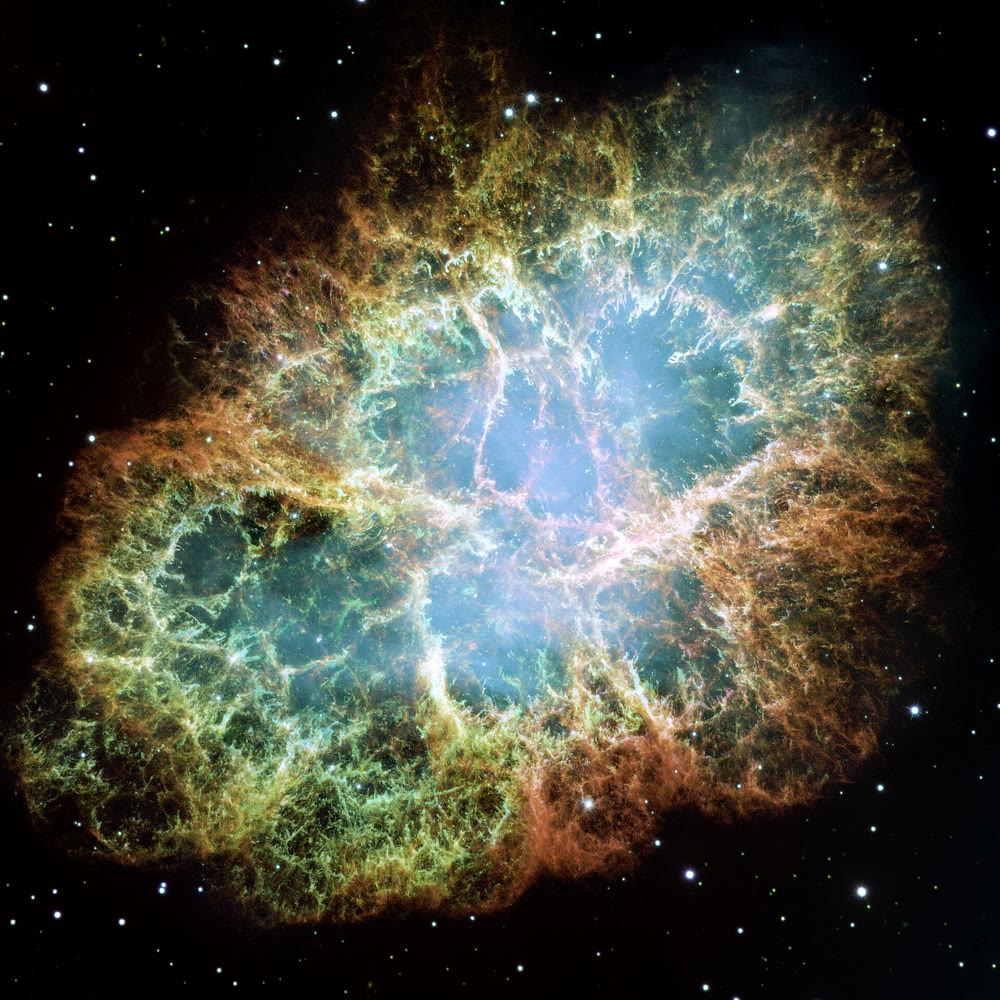
\includegraphics[width=0.45\linewidth]{images/book1/crab-nebula.jpg}

{\small A Nebulosa do Caranguejo, a nuvem deixada por uma estrela que
explodiu há quase mil anos, espalhando novos elementos pelo espaço
(NASA, ESA, J.~Hester e A.~Loll).}
\end{omfigure}

\section{A Terra}

\begin{proposition}[A crosta terrestre]\label{prop:g9:elements-universe-earth:crust}
% ledger: ab:crust-O, ab:crust-Si, ab:crust-Al, ab:crust-Fe, ab:crust-Ca, ab:crust-Na, ab:crust-K, ab:crust-Mg, ab:crust-first10
A fina pele rochosa da Terra, a crosta, tem em massa quase metade de
oxigênio e mais de um quarto de silício: as rochas e a areia são
principalmente óxidos de silício e de alguns \omterm{def:g9:periodic-table-first-look:metal}{metais}. Oito elementos ---
oxigênio, silício, alumínio, ferro, cálcio, sódio, potássio, magnésio
--- formam cerca de \qty{99}{\percent} dela. O hidrogênio e o hélio, tão
comuns nas estrelas, são raros: os gases leves escaparam da Terra
jovem.
\end{proposition}

\begin{remark}[Dentro da Terra]\label{rem:g9:elements-universe-earth:core}
A crosta não é a Terra inteira. O ferro, pesado, afundou em direção ao
centro quando a Terra jovem estava derretida: o \omterm{def:g9:inside-the-atom:nucleus}{núcleo} da Terra é
principalmente ferro, com um pouco de níquel.
\end{remark}

\begin{proposition}[Os oceanos e o ar]\label{prop:g9:elements-universe-earth:ocean}
% ledger: sea:salts-share, sea:NaCl-ions, sea:MgSO4-ions, air:N2, air:O2
A água do mar é principalmente água --- hidrogênio e oxigênio --- com
cerca de \qty{3.5}{\percent} de sais dissolvidos em massa. Entre os \omterm{def:g9:ions:ion}{íons}
dissolvidos, o cloreto e o sódio formam cerca de \qty{85}{\percent}, o
magnésio e o sulfato outros \qty{10}{\percent}. O \omterm{def:g4:air-a-mixture-of-gases:air}{ar} é principalmente
nitrogênio e oxigênio.
\end{proposition}

\begin{omfigure}
\begin{tikzpicture}
\begin{axis}[xbar, width=0.40\linewidth, height=5.4cm, xmin=0, xmax=85,
    bar width=7pt, symbolic y coords={Mg,K,Na,Ca,Fe,Al,Si,O}, ytick=data,
    xlabel={porcentagem da massa}, title={\small a crosta terrestre},
    nodes near coords, nodes near coords style={font=\scriptsize},
    tick label style={font=\small}, label style={font=\small},
    axis lines*=left, enlarge y limits=0.08]
% ledger: ab:crust-O, ab:crust-Si, ab:crust-Al, ab:crust-Fe, ab:crust-Ca, ab:crust-Na, ab:crust-K, ab:crust-Mg
\addplot[fill=omDef!45, draw=omDef] coordinates {(46.6,O) (27.7,Si) (8.1,Al)
  (5.0,Fe) (3.6,Ca) (2.8,Na) (2.6,K) (2.1,Mg)};
\end{axis}
\end{tikzpicture}\hfill
\begin{tikzpicture}
\begin{axis}[xbar, width=0.40\linewidth, height=5.4cm, xmin=0, xmax=85,
    bar width=7pt, symbolic y coords={{P},{N},{Ca},{H},{C},{O}}, ytick=data,
    xlabel={porcentagem da massa}, title={\small um corpo humano},
    nodes near coords, nodes near coords style={font=\scriptsize},
    tick label style={font=\small}, label style={font=\small},
    axis lines*=left, enlarge y limits=0.1]
% ledger: body:atoms-O, body:atoms-C, body:atoms-H, body:atoms-N, body:atoms-Ca, body:atoms-P (masses = atoms x atomic mass, over 70 kg)
\addplot[fill=omProp!45, draw=omProp] coordinates {(61.1,O) (22.9,C) (10.1,H)
  (1.3,N) (1.5,Ca) (0.7,P)};
\end{axis}
\end{tikzpicture}

{\small \omterm{def:g9:elements-universe-earth:abundance}{Abundâncias} em massa. À esquerda: os oito principais elementos
da crosta terrestre. À direita: os seis principais elementos do corpo de
um adulto magro (calculados a partir de números estimados de \omterm{def:g7:atoms-and-molecules:atom}{átomos}).}
\end{omfigure}

\section{O corpo humano}

\begin{proposition}[De que somos feitos]\label{prop:g9:elements-universe-earth:body}
% ledger: body:atoms-O, body:atoms-C, body:atoms-H, body:atoms-N, body:atoms-Ca, body:atoms-P, body:atoms-total
Em massa, o corpo de um adulto magro tem cerca de \qty{61}{\percent} de
oxigênio, \qty{23}{\percent} de carbono e \qty{10}{\percent} de
hidrogênio --- principalmente na água e nas \omterm{def:g7:atoms-and-molecules:molecule}{moléculas} da vida ---,
seguidos pelo nitrogênio, pelo cálcio (nos ossos e nos dentes) e pelo
fósforo. Contando em \omterm{def:g7:atoms-and-molecules:atom}{átomos} e não em massa, a ordem muda: há mais
\omterm{def:g7:atoms-and-molecules:atom}{átomos} de hidrogênio num corpo do que todos os outros \omterm{def:g7:atoms-and-molecules:atom}{átomos} juntos,
porque os \omterm{def:g7:atoms-and-molecules:atom}{átomos} de hidrogênio são muito leves. Um corpo de
\qty{70}{kg} contém cerca de $7 \times 10^{27}$ \omterm{def:g7:atoms-and-molecules:atom}{átomos}.
\end{proposition}

\begin{method}[Ler um gráfico de abundâncias]\label{met:g9:elements-universe-earth:read}
\begin{enumerate}
  \item Verifique o que é medido: a massa (na maioria dos gráficos) ou o
        número de \omterm{def:g7:atoms-and-molecules:atom}{átomos}.
  \item Leia a parte de cada elemento; some as dos principais para ver
        quanto eles cobrem.
  \item Para comparar dois corpos, procure os elementos comuns aos dois
        e os que só aparecem num deles.
\end{enumerate}
O oxigênio está no topo dos dois gráficos deste capítulo: ele é o
elemento mais comum da crosta e do corpo humano, em massa.
\end{method}

\section{Os mesmos átomos, reciclados}

\begin{example}[A viagem de um átomo de carbono]\label{ex:g9:elements-universe-earth:journey}
Um \omterm{def:g7:atoms-and-molecules:atom}{átomo} de carbono fabricado numa estrela há muito tempo pode ficar
milhões de anos num calcário, ser liberado como dióxido de carbono por
um vulcão, ser absorvido por uma folha, virar parte de um açúcar numa
fruta, passar para um animal que come a fruta e ser expirado de novo
como dióxido de carbono. Os \omterm{def:g7:atoms-and-molecules:atom}{átomos} não são destruídos pelas
\omterm{def:g5:irreversible-changes:chemical-change}{transformações químicas}: eles são passados adiante.
\end{example}

\begin{omfigure}
\begin{tikzpicture}[font=\small,
    box/.style={draw=omDef, fill=omDef!6, rounded corners=2pt, align=center,
      minimum height=0.85cm, text width=2.3cm}]
  \node[box] (a) at (0,2.2) {numa rocha\\ (calcário)};
  \node[box] (b) at (4.3,2.2) {no ar\\ (\ce{CO2})};
  \node[box] (c) at (8.6,2.2) {numa folha\\ (açúcar)};
  \node[box] (d) at (8.6,0) {num animal};
  \node[box] (e) at (4.3,0) {expirado\\ (\ce{CO2})};
  \draw[->, thick, omProp] (a) -- node[above, font=\footnotesize] {vulcão} (b);
  \draw[->, thick, omProp] (b) -- (c);
  \draw[->, thick, omProp] (c) -- node[right, font=\footnotesize] {comido} (d);
  \draw[->, thick, omProp] (d) -- (e);
  \draw[->, thick, omProp] (e) -- (b);
\end{tikzpicture}

{\small Um \omterm{def:g7:atoms-and-molecules:atom}{átomo} de carbono passa da rocha para o \omterm{def:g4:air-a-mixture-of-gases:air}{ar}, do \omterm{def:g4:air-a-mixture-of-gases:air}{ar} para a folha,
da folha para o animal e de volta para o \omterm{def:g4:air-a-mixture-of-gases:air}{ar}: o próprio \omterm{def:g7:atoms-and-molecules:atom}{átomo} nunca é
destruído.}
\end{omfigure}

\begin{omfigure}
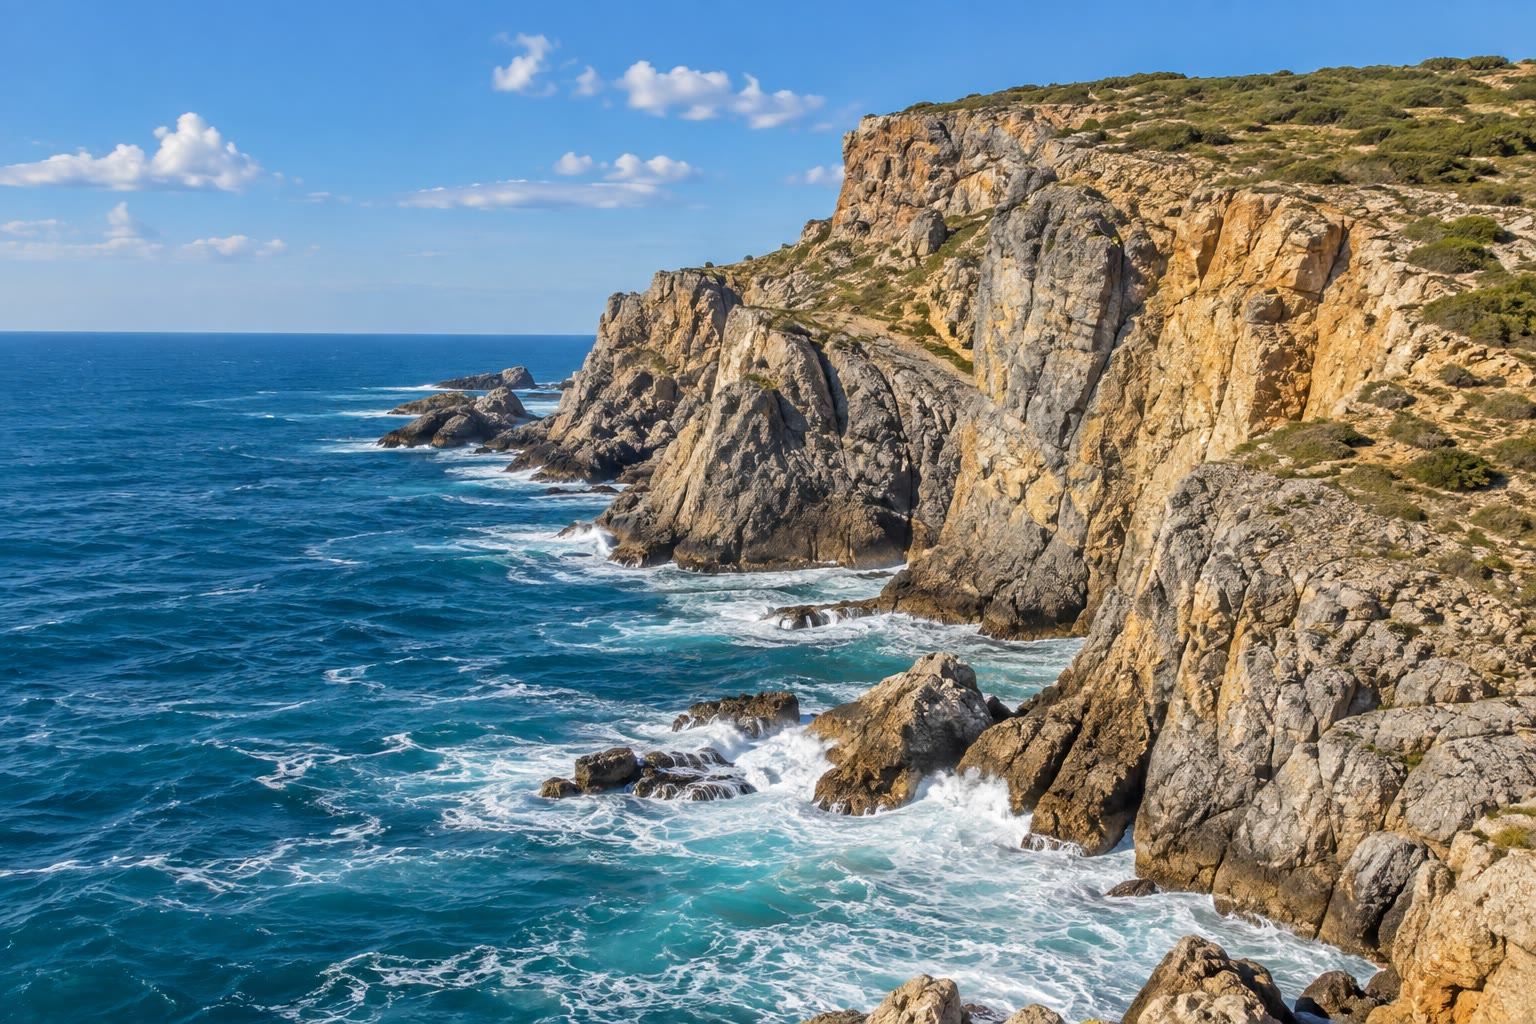
\includegraphics[width=0.55\linewidth]{images/book1/ai/g9-coastal-cliff.jpg}

{\small Rocha, mar e \omterm{def:g4:air-a-mixture-of-gases:air}{ar}: três \omterm{def:g6:pure-substances-and-mixtures:mixture}{misturas} muito diferentes dos mesmos
elementos.}
\end{omfigure}

\section{Exercícios}

\begin{exercise}[$\star$]\label{exo:g9:elements-universe-earth:1}
Que dois elementos formam quase todo o Sol?
\end{exercise}

\begin{exercise}[$\star$]\label{exo:g9:elements-universe-earth:2}
Qual é o elemento mais abundante na crosta terrestre? E no corpo humano
(em massa)?
\end{exercise}

\begin{exercise}[$\star$]\label{exo:g9:elements-universe-earth:3}
Onde foi fabricada a maioria dos elementos mais pesados que o hélio?
\end{exercise}

\begin{exercise}[$\star$]\label{exo:g9:elements-universe-earth:4}
Que porcentagem da massa da água do mar é sal dissolvido?
\end{exercise}

\begin{exercise}[$\star\star$]\label{exo:g9:elements-universe-earth:5}
Usando o gráfico da crosta, some as partes do oxigênio e do silício. Que
fração da crosta é isso, aproximadamente?
\end{exercise}

\begin{exercise}[$\star\star$]\label{exo:g9:elements-universe-earth:6}
Por que há tão pouco hidrogênio e hélio na crosta terrestre, se o Sol é
feito quase inteiramente deles?
\end{exercise}

\begin{exercise}[$\star\star$]\label{exo:g9:elements-universe-earth:7}
Que massa de carbono há num corpo de \qty{70}{kg} que tem
\qty{23}{\percent} de carbono?
\end{exercise}

\begin{exercise}[$\star\star$]\label{exo:g9:elements-universe-earth:8}
Por que o oxigênio é o elemento mais comum do corpo em massa, enquanto o
hidrogênio é o mais comum em número de \omterm{def:g7:atoms-and-molecules:atom}{átomos}?
\end{exercise}

\begin{exercise}[$\star\star$]\label{exo:g9:elements-universe-earth:9}
Um bloco de granito de \qty{1000}{kg} é um pedaço típico da crosta.
Usando o gráfico, mais ou menos que massa de alumínio ele contém?
\end{exercise}

\begin{exercise}[$\star\star$]\label{exo:g9:elements-universe-earth:10}
Que elementos aparecem entre os principais elementos tanto da crosta
quanto do corpo humano?
\end{exercise}

\begin{exercise}[$\star\star\star$]\label{exo:g9:elements-universe-earth:11}
Um corpo de \qty{70}{kg} contém cerca de \qty{1.06}{kg} de cálcio.
Calcule a massa de um \omterm{def:g7:atoms-and-molecules:atom}{átomo} de cálcio ($A = 40$), e depois o número de
\omterm{def:g7:atoms-and-molecules:atom}{átomos} de cálcio. Escreva-o em notação científica.
\end{exercise}

\begin{exercise}[$\star\star\star$]\label{exo:g9:elements-universe-earth:12}
Os \omterm{def:g7:atoms-and-molecules:atom}{átomos} do seu corpo já fizeram parte de outras coisas antes. Use a
viagem de um \omterm{def:g7:atoms-and-molecules:atom}{átomo} de carbono para explicar por que o número total de
\omterm{def:g7:atoms-and-molecules:atom}{átomos} de carbono na Terra quase não muda.
\end{exercise}

\section{Problema: quantos átomos eu sou?}

\begin{problem}[{Problema de fim de semana --- de um gráfico de
abundâncias até o número de átomos de oxigênio num corpo humano}]
\label{pb:g9:elements-universe-earth:1}
% ledger: body:atoms-O, body:atoms-total
Um adulto magro de \qty{70}{kg} tem, em massa, cerca de
\qty{61}{\percent} de oxigênio, \qty{23}{\percent} de carbono e
\qty{10}{\percent} de hidrogênio. Tome a massa de um \omterm{def:g9:inside-the-atom:proton}{núcleon} como
\qty{1.67e-27}{kg}; um \omterm{def:g7:atoms-and-molecules:atom}{átomo} de oxigênio tem 16 \omterm{def:g9:inside-the-atom:proton}{núcleons}, um \omterm{def:g7:atoms-and-molecules:atom}{átomo} de
carbono 12, um \omterm{def:g7:atoms-and-molecules:atom}{átomo} de hidrogênio 1. Os \omterm{def:g9:inside-the-atom:nucleus}{elétrons} são desprezados.

\medskip
\noindent\textbf{Parte I --- As massas.}
\begin{enumerate}
  \item Calcule a massa de oxigênio no corpo.
  \item Calcule a massa de carbono e a de hidrogênio.
  \item Que porcentagem da massa esses três elementos formam juntos?
  \item A maior parte desse oxigênio e desse hidrogênio está num único
        composto. Qual?
\end{enumerate}

\medskip
\noindent\textbf{Parte II --- Um \omterm{def:g7:atoms-and-molecules:atom}{átomo}.}
\begin{enumerate}[resume]
  \item Calcule a massa de um \omterm{def:g7:atoms-and-molecules:atom}{átomo} de oxigênio.
  \item Calcule a massa de um \omterm{def:g7:atoms-and-molecules:atom}{átomo} de carbono e a de um \omterm{def:g7:atoms-and-molecules:atom}{átomo} de
        hidrogênio.
  \item Quantos \omterm{def:g7:atoms-and-molecules:atom}{átomos} de hidrogênio pesam tanto quanto um \omterm{def:g7:atoms-and-molecules:atom}{átomo} de
        oxigênio?
  \item Por que os \omterm{def:g9:inside-the-atom:nucleus}{elétrons} podem ser desprezados?
\end{enumerate}

\medskip
\noindent\textbf{Parte III --- A contagem.}
\begin{enumerate}[resume]
  \item Calcule o número de \omterm{def:g7:atoms-and-molecules:atom}{átomos} de hidrogênio no corpo.
  \item Calcule o número de \omterm{def:g7:atoms-and-molecules:atom}{átomos} de carbono.
  \item Calcule o número de \omterm{def:g7:atoms-and-molecules:atom}{átomos} de oxigênio no corpo.
  \item Uma estimativa cuidadosa dá $1.61 \times 10^{27}$ \omterm{def:g7:atoms-and-molecules:atom}{átomos} de
        oxigênio num corpo assim. Compare com a sua contagem, e dê o
        número de \omterm{def:g7:atoms-and-molecules:atom}{átomos} de oxigênio num corpo de \qty{70}{kg} com dois
        algarismos significativos.
\end{enumerate}
\end{problem}
